%% fancy header & foot
\pagestyle{fancy}
\lhead{[ELEC-H-2001] Électricité\\ TP \no 2 : Circuits réactifs avec sources de tension continue\ifthenelse{\boolean{corrige}}{~-- corrigé}{}}
\rhead{v1.0.1\\ page \thepage}
\cfoot{}
%%

\pdfinfo{
/Author (Raoul Sommeillier, ULB -- BEAMS)
/Title (TP 2 ELEC-H-2001, Circuits réactifs avec sources de tension continue)
/ModDate (D:\pdfdate)
}

\hypersetup{
pdftitle={TP 2 [ELEC-H-2001] Électricité : Circuits réactifs avec sources de tension continue},
pdfauthor={Raoul Sommeillier, ©2018 ULB - BEAMS  },
%pdfsubject={filtrage et analyse fréquentielle}
}

%\date{\vspace{-1cm}\mydate\today}
%\title{\vspace{-2cm} Labo \no 6\\ Électronique appliquée [ELEC-H-301]\\Réalisation d'un ampli à transistor\ifthenelse{\boolean{corrige}}{~\\Corrigé}{}}

%\author{\vspace{-1cm}}%\textsc{Yannick Allard}}

\setlength{\parskip}{0.5cm plus4mm minus3mm} %espacement entre §
\setlength{\parindent}{0pt}


\begin{document}

\tptitle{}{Séance 2~: Circuits réactifs avec sources de tension continue}

\section{Pré-requis}
Avant la séance, vous aurez lu attentivement l’énoncé de la manipulation. Vous aurez par ailleurs relu les chapitres et sections suivants:
\begin{itemize}
	\item Chapitre 6 - Résoudre un circuit réactif dans le domaine temporel 
	\begin{itemize}
	\item Section 6.1 - Eléments réactifs : rappels  (jusqu’aux lois court et long termes)
	\item Section 6.2 - Analyse temporelle du circuit RC 
	\item Section 6.3 - Analyse temporelle du circuit RL
	\item Section 6.6 - Analyse temporelle du circuit RLC
	\end{itemize}
\end{itemize}

\vspace{5pt}

\newpage

\section{Exercices}
\subsection{RC 1}
%\ifthenelse{\boolean{assistant}}
%{\color{blue} Exercice prioritaire \\ Timing: 15min \\
%
%Le but de cet exercice est d’habituer les étudiants à reconnaître des courbes de tension et de courant relatives à un circuit réactif. On s’attend à une certaine confusion entre le comportement d’une inductance et d’une capacité, ce que cet exercice vise à éliminer.  En fin d’exercice, insister sur la différence entre ces deux composants en courant et en tension. L’influence de la charge initiale est étudiée.\\ \color{black}}{}


Considérer le circuit suivant, avec E=120V : 
\begin{center}
\begin{circuitikz} \draw
(0,0)	to[battery1, l=$E$, invert]	(0,3)
		to[closing switch, l=$t_0$] (3,3)
		to[C, l=$C$]		(3,1.5)
		to[R, l=$R$]		(3,0)--(0,0)
;
\end{circuitikz}
\end{center}

Avant $t=0$, l’interrupteur est ouvert. La charge initiale de la capacité est nulle. On ferme l’interrupteur à l’instant $t=0$. \\

On relève les deux courbes suivantes (temps en abscisse, tension ou courant en ordonnée):
\begin{center}
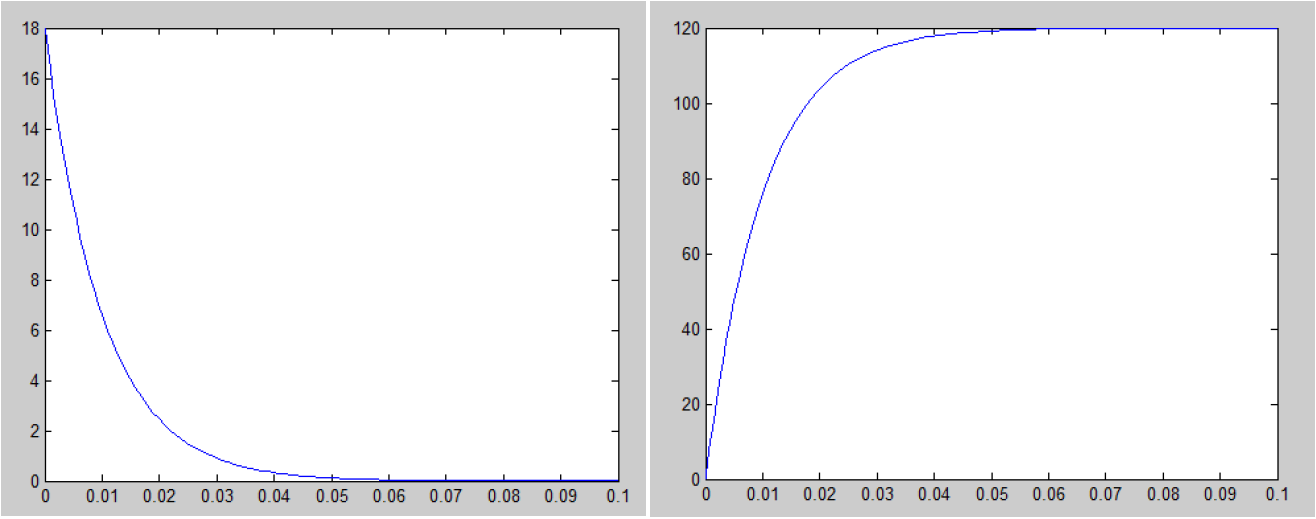
\includegraphics[scale=0.4]{TP2/TP2-Exo1a.PNG}
\end{center}

\Question
{
%question
\textit{Identifier l'élément du schéma (source E, capacité, résistance) auquel se rapportent ces deux graphes.}
}
{%correction
Attention, la réponse n'est valable que si l'on définit correctement la tension et le courant (module et sens):
\begin{center}
\begin{circuitikz} \draw
(0,0)	to[battery1, v=$E$, i^>=$i$, invert]	(0,3)
		to[closing switch, l=$t_0$] (3,3)
		to[C, l_=$C$, v^<=$V_C$]		(3,1.5)
		to[R, l=$R$]		(3,0)--(0,0)
;
\end{circuitikz}
\end{center}
La courbe de gauche représente le courant selon le sens choisi sur le schéma (en termes de forme, elle pourrait aussi représenter la ddp sur la résistance, mais dans ce cas la valeur de départ devrait être 120: il s'agit donc du courant) . La courbe de droite représente la ddp sur la capacité selon le sens choisi sur le schéma. Les valeurs initiales et finales sont importantes, ainsi que les asymptotes horizontales.
}


\Question
{
%question
\textit{Identifier la grandeur (tension(s), courant(s) ?) présente sur l'ordonnée de chaque graphe.}
}
{%correction
Sur la courbe de gauche, la valeur 18 représente un courant initial de 18A. En effet, le courant peut varier instantanément pour une capacité. Dans ce cas, il vaut simplement $\frac{120}{R}$, ce qui mène à $R=\frac{120}{18} \Omega$.\\
Sur la courbe de droite, 120 représente la tension de régime que va atteindre la capacité. En effet, suivant l'équation de maille $E=V_{C}+RI$, étant donné que le courant sera nul en régime (loi BF d'une capacité), la tension $V_{C}$ sera alors égale à $E$. 
Lors d'une autre mesure, la courbe suivante est relevée:
\begin{center}
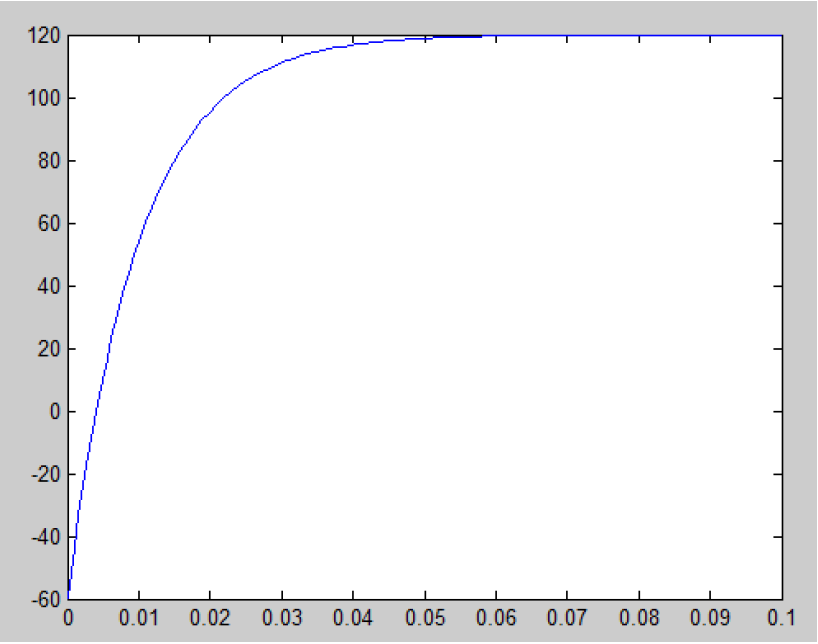
\includegraphics[scale=0.4]{TP2/TP2-Exo1b.PNG}
\end{center}
}

\Question
{
%question
\textit{Que représente-t-elle? Exliquer la présence de valeurs négatives et positives pour cette grandeur.}
}
{%correction
La courbe représente la tension aux bornes de la capacité. La charge initiale de celle-ci est telle que la tension est de -60V si on respecte le sens suivant pour la tension sur la capacité.
\begin{center}
\begin{circuitikz} \draw
(0,0)	to[battery1, v=$E$, i^>=$i$, invert]	(0,3)
		to[closing switch, l=$t_0$] (3,3)
		to[C, l_=$C$, v^<=$V_C$]		(3,1.5)
		to[R, l=$R$]		(3,0)--(0,0)
;
\end{circuitikz}
\end{center}
Il est intéressant de noter que la tension aux bornes de la capacité ne met pas plus de temps à atteindre sa valeur de régime lorsqu'elle a une charge initiale négative. En effet, ce temps est déterminé grâce à la constante de temps $\tau=RC$ qui est indépendante de la charge initiale.
}

\Question
{
%question
\textit{Si la capacité était remplacée par une inductance, quelle serait l'allure du courant du circuit et de la tension aux bornes de l'inductance?}
}
{%correction
L'allure de la tension aux bornes de l'inductance est d'allure semblable à celle du courant du circuit avec la capacité, et l'allure du courant dans le circuit avec l'inductance est semblable à celle de la tension aux bornes de la capacité.
}


\subsection{RC 2}
\Question
{
%question
\textit{Une capacité peut-elle fournir de l'énergie à un circuit?}
}
{%correction
Oui, elle peut restituer l'energie qu'elle a emmagasinée. Il s'agit de la tension initiale $V(0)$ qui agit alors comme une source qui fournit de l'énergie.
}

\begin{center}
\begin{circuitikz} \draw
(0,0)	to[battery1, v=$E$, invert]	(0,3)
		to[R, l_=$R$, v^<=$V_R$]		(3,3)
		to[C, l_=$C$, v^<=$V_C$]		(3,0)--(0,0)
;
\end{circuitikz}
\end{center}

\Question
{
%question
\textit{Pour le circuit suivant, est-il correct d'écrire:}\\
$$ V_{C}(t)=V(0)+\int_{0}^{t}\frac{1}{C}i(\xi)d\xi \hspace{1cm} ou \hspace{1cm} V_{C}(t)=V(0)-\int_{0}^{t}\frac{1}{C}i(\xi)d\xi \hspace{1cm} ?$$
}
{%correction
Pour répondre à cette question, il faut définir le sens du courant, sinon les deux expressions de $V_{C}$ ci-dessus n'ont aucun sens.
\begin{center}
\begin{circuitikz} \draw
(0,0)	to[battery1, v=$E$, i^>=$i$, invert]	(0,3)
		to[R, l_=$R$, v^<=$V_R$]		(3,3)
		to[C, l_=$C$, v^<=$V_C$]		(3,0)--(0,0)
;
\end{circuitikz}
\end{center}
Dans le cas ci-dessus, et en supposant $V(0)$ défini dans le même sens que $V_{C}$, la bonne expression est: 
$$V_{C}(t)=V(0)+\int_{0}^{t}\frac{1}{C}i(\xi)d\xi $$

Si le courant est défini dans le même sens que la tension par rapport à la capacité:
\begin{center}
\begin{circuitikz} \draw
(0,0)	to[battery1, v=$E$, i<=$i$, invert]	(0,3)
		to[R, l_=$R$, v^<=$V_R$]		(3,3)
		to[C, l_=$C$, v^<=$V_C$]		(3,0)--(0,0)
;
\end{circuitikz}
\end{center}
L'expression correcte est alors:\\
$$V_{C}(t)=V(0)-\int_{0}^{t}\frac{1}{C}i(\xi)d\xi $$
}


\subsection{RL}
%\ifthenelse{\boolean{assistant}}
%{\color{blue} Cet exercice n'est pas prioritaire.\\
%
%$\rightarrow$ Le but est de convaincre les étudiants que la loi $V=RI$ ne doit pas être utilisée pour tous les éléments. Il s’agit d’un raisonnement faux qui se base sur $V=RI$ appliqué  à une inductance. L’étudiant doit différencier la notion de modèle et d’élément réel (un fil a une certaine inductance et une bobine a une certaine résistance donc la discussion dépend du contexte). \\ \color{black}}{}


Pour le circuit suivant:
\begin{center}
\begin{circuitikz} \draw
(0,0)	to[battery1, v=$E$, invert]	(0,3)
		to[R, l_=$R$]		(3,3)
		to[L, l_=$L$]		(3,0)--(0,0)
;
\end{circuitikz}
\end{center}
\textit{Étant donné qu'une inductance est fondamentalement un fil bobiné d'une façon particulière, la loi d'Ohm peut lui être appliquée. Or, en régime, comme la tension sur une inductance est nulle, on en conclut que, pour le circuit suivant, $i=0A$ en régime.}

\Question
{
%question
\textit{Expliquer pourquoi ce raisonnement (écrit en italique) est erroné.}
}
{%correction
Dans un schéma comme ci-dessus, R et L sont des dipôles idéaux. L'élément L est donc par définition une inductance pure répondant à la loi $V(t) = L \frac{di}{dt}$ et rien d'autre (il ne comprend en particulier pas de partie résistive). \\
Lorsque le texte évoque une inductance comme étant un fil bobiné, il évoque la version réelle d'une inductance, qu'on appellera plutôt une "bobine". Cette bobine possède à la fois un comportement inductif (comme une inductance pure) et un comportement résistif dû à la résistance du fil qui la constitue. Elle peut, dans sa globalité, être modélisée par l'ensemble R+L tel que dans le schéma ci-dessus. La bobine réelle est donc représentée ci-dessus par l'association d'une résistance pure et d'une inductance pure.\\
L'erreur du raisonnement est donc de confondre inductance réelle et inductance idéale: comme L dans le schéma représente une inductance idéale, la loi d'Ohm V=RI ne lui est pas applicable. Le fait que la tension soit nulle en régime sur L permet seulement de conclure que le courant sera constant en régime. (Il vaudra en particulier $E/R$)
}

\subsection{Du circuit aux équations}
%%assistant
%
%\ifthenelse{\boolean{assistant}}
%{\color{blue} Cet exercice n'est pas prioritaire.\\
%
%$\rightarrow$ Le but est de les habituer à différencier le comportement des inductances du comportement des capacités. Les conditions initiales pour la résolution d’équations différentielles semblent être un point sensible à l’examen. Le focus devrait donc être sur les conditions initiales.\\ \\ \color{black}}{}

Pour le circuit suivant:
\begin{center}
\begin{circuitikz} \draw
(0,0)	to[battery1, v=$E$, invert]			(0,4)
		to[closing switch, l=$t_0$] (2,4)
		to[C, l=$C$]				(2,2)
		to[R, l=$R_1$]				(2,0)
(2,4)--(4,4)
		to[L, l=$L$]				(4,2)
		to[R, l=$R_2$]				(4,0)--(0,0)
;
\end{circuitikz}
\end{center}

\Question
{
%question
\textit{Écrire les équations du circuit avant et après fermeture (fermeture en t=0) de l'interrupteur qui permettent de trouver les tensions et courants de tous les éléments.}
}
{%correction
Attention : ne pas oublier d'analyser ce qui se passe pour $t<0$, qui peut être très différent du comportement pour $t>0$. 

D'abord, on définit les courants et tensions en module et sens:
\begin{center}
\begin{circuitikz} \draw
(0,0)	to[battery1, v=$E$, i^>=$i_{tot}$, invert]			(0,4)
		to[closing switch, l=$t_0$] (2,4)
		to[C, l=$C$, v<=$V_C$, i=$i_1$]				(2,2)
		to[R, l=$R_1$, v<=$V_{R_1}$]				(2,0)
(2,4)--(4,4)
		to[L, l=$L$, i=$i_2$, v<=$V_L$]				(4,2)
		to[R, l=$R_2$, v<=$V_{R_2}$]				(4,0)--(0,0)
;
\end{circuitikz}
\end{center}
On peut alors faire le raisonnement suivant.

Avant la fermeture: l'interrupteur étant ouvert, la source de tension E est déconnectée des deux autres branches verticales du circuit et ne les influence pas. Dans l'absolu ceci ne veut pas dire qu'il ne peut pas y avoir de tension ou de courant dans ces branches. Cependant on peut observer que L et C sont en série (s'il y a un courant dans L c'est forcément le même dans C: $i_1 = -i_2$), or à long terme le courant est nul dans une capacité. Tous les courants sont donc nuls. En conséquence la ddp est nulle sur L et sur les deux R. Et comme ces trois éléments forment avec C une maille sur laquelle la tension totale doit être nulle, la ddp sur C est forcément nulle également. \\
Avant la fermeture, toutes les grandeurs électriques sont donc nulles dans les deux branches de droite. \\
N.B.: La ddp sur l'interrupteur vaut E pour vérifier la loi des mailles dans la maille de gauche.\\

Après fermeture :
$$E=V_{C}+V_{R_1}=V_{C}(0)+\int_{0}^{t}\frac{1}{C}i_1(\xi)d\xi+R_1i_{1}$$
$$E=V_{L}+V_{R_2}=L\frac{di_{2}}{dt}+R_2 i_{2}$$

Si l'on ne souhaite pas d'intégrale, on peut aussi écrire la première équation:
$$E=V_{C}+V_{R_1}=V_C+R_1 i_1=V_C + R_1 C\frac{dV_C}{dt}$$
}
\Question
{
%question
\textit{Donner les conditions initiales nécessaires à la résolution de ces équations.}
}
{%correction
Le courant dans l'inductance ne peut pas changer instantanément (loi HF d'une inductance):
$$i_{2}^{0+}=i_{2}^{0-}$$\\
et la tension aux bornes de la capacité ne peut pas changer instantanément (loi HF d'une capacité):
$$V_{C}^{0+}=V_{C}^{0-}$$\\
}

\subsection{Analyse qualitative}
%\ifthenelse{\boolean{assistant}}
%{\color{blue} Cet exercice n'est pas prioritaire.\\
%
%$\rightarrow$ Le but de cet exercice est d’étudier l’effet d’une résistance court-circuitée dans un circuit inductif. On s’attend à ce que l’étudiant pense qu’étant donné la présence d’une inductance dans le circuit, il est légitime de supposer que les courants i1 et i2 ne peuvent pas évoluer brutalement alors que c’est le courant total qui est soumis à la continuité du courant dans l’inductance.\\ \\ \color{black}}{}

Pour le circuit suivant:
\begin{center}
\begin{circuitikz} \draw
(0,0)	to[battery1, l=$E$, invert]			(0,6)
		to[closing switch, l=$t_0$, i=$i_1$]	(6,6)--(6,4)
		to[R, l=$R_2$]				(6,2)
		to[L, l=$L$]				(6,0)--(0,0)
(1,6)--(1,4)
		to[R, l=$R_1$, i=$i_2$]				(5,4)--(5,6)
;
\end{circuitikz}
\end{center}
Pour $t<0$, l'interrupteur est en position ouverte et le circuit est en régime. On ferme l'interrupteur à l'instant $t=t_0=0$, et on s'intéresse ensuite au temps $t>0$.

\Question
{
%question
\textit{Indiquer si les deux phrases suivantes sont correctes et justifier.
\begin{enumerate}
\item	La résistance totale du circuit (vue de la source) diminue après la fermeture de l'interrupteur.
\item	Étant donné qu'il y a une inductance dans le circuit:
	\begin{itemize}
	\item  le courant $i_{2}$ ne peut pas s'annuler directement lors de la fermeture du circuit: il passera (au signe près) progressivement de $\frac{E}{R_{1}+R_{2}}$ à $0A$.
	\item 	le courant $i_{1}$ passera immédiatement (au signe près) de $0 A$ à $\frac{E}{R_{2}}$ 	
	\end{itemize}
\end {enumerate}}
}
{%correction
\begin{enumerate}
\item	\textit{La résistance totale du circuit (vue de la source) diminue après la fermeture de l'interrupteur.}\\
%corrigé
La résistance totale du circuit passe de $R_{1}+R_{2}$ à $R_{2}$ étant donné qu'à partir de $t=0$, $R_{1}$ est court-circuitée. Le schéma équivalent de $R_1$ en parallèle avec l'interrupteur fermé est un court-circuit. Par conséquent, la résistance $R_{1}$ n'a plus aucun effet lors de l'étude du circuit, et l'affirmation est correcte.  
%fin corrigé
\item	\textit{Étant donné qu'il y a une inductance dans le circuit:}
\begin{itemize}
\item  \textit{le courant $i_{2}$ ne peut pas s'annuler directement lors de la fermeture du circuit: il passera (au signe près) progressivement de $\frac{E}{R_{1}+R_{2}}$ à $0A$.}\\
%corrigé
Le courant $i_{2}$ va s'annuler dès le moment où l'interrupteur est fermé ; il n'y a en effet aucune inductance dans cette partie du circuit. C'est en effet uniquement le courant qui parcourt l'inductance qui est régi par la loi de la continuité du courant.
\item 	\textit{le courant $i_{1}$ passera immédiatement (au signe près) de $0 A$ à $\frac{E}{R_{2}}$.}\\
%corrigé
Le courant $i_{1}$ va immédiatement passer de zéro à $\frac{E}{R1+R2}$ en $t=0$ étant donné que le courant dans une inductance est régi par

$$i_{inductance}^{0+}=i_{inductance}^{0-}$$

Il ne va donc pas prendre la valeur $\frac{E}{R_{2}}$ directement. Il s'agira de sa valeur de régime.
Le courant $i_{1}$ va donc passer directement de $0$ à $\frac{E}{R1+R2}$ étant donné qu'il s'agit du courant qui passe dans l'inductance avant fermeture et qu'il respecte la continuité du courant dans une inductance. Il va ensuite, à partir de cette valeur $\frac{E}{R1+R2}$, passer progressivement à sa valeur de régime $\frac{E}{R_{2}}$.
	\end{itemize}
\end {enumerate}
}

\subsection{Analyse et résolution d'un circuit}
%\ifthenelse{\boolean{assistant}}
%{\color{blue} Cet exercice n'est pas prioritaire.\\
%
%$\rightarrow$ Le but est de permettre aux étudiants de résoudre de A à Z un circuit réactif. Les trois premières questions font réaliser à l’étudiant que certains principes peuvent être utilisés afin de vérifier leurs résultats analytiques obtenus par la suite. Il est important de résoudre l’équation différentielle avec eux puisque cela requiert les conditions initiales. On s’attend également à ce que les étudiants appliquent les conditions initiales avant d’avoir trouvé la solution particulière.\\ \color{black}}{}

Pour t<0, le circuit suivant est en régime avec l'interrupteur ouvert. On ferme l'interrupteur en t=0.
\begin{center}
\begin{circuitikz} \draw
(0,0)	to[battery1, l=$E$, invert]			(0,2)
		to[R, l=$R_1$]				(2,2)
		to[closing switch, l=$t_0$]	(4,2)
		to[R, l=$R_2$]				(4,0)--(0,0)
(2,2)	to[C, l=$C$]				(2,0)
;
\end{circuitikz}
\end{center}

\Question
{
%question
\textit{Une capacité peut-elle se charger indéfiniment?}
}
{%correction
Non, que ce soit à cause de la topologie du circuit ou des limites physiques de la capacité.
}

\Question
{
%question
\textit{Que vaudra, en régime (avec l'interrupteur fermé), la tension aux bornes de la résistance $R_{2}$?}
}
{%correction
En régime, il n'y a pas de courant qui passe dans la capacité (loi BF). L'unique courant restant parcourra la maille comprenant la source de tension et les résistances $R_{1}$ et $R_{2}$ en série.\\
Nous avons donc $i=\frac{E}{R_{1}+R_{2}}$\\
La tension aux bornes de la résistance $R_{2}$ vaut $V_{R_{2}}=R_{2}i$\\
Ce qui nous donne  $V_{R_{2}}=E\frac{R_{2}}{R_{1}+R_{2}}$
}

\Question
{
%question
\textit{Est-il correct de dire que la condition initiale, en t=0, est exprimée par la tension nulle sur la résistance $R_{2}$ suivant le raisonnement suivant :\\
\og Le courant total de régime, au moment où l’interrupteur est fermé, est nul, puisqu’avant de fermer l’interrupteur, le circuit est en régime. Or, en régime, une capacité est analogue à un circuit ouvert. Comme $V=RI$ et qu'il n'y a pas de courant, la tension sur $R_{2}$ est bien nulle.\fg}
}
{%correction
C’est faux. La condition qu’impose la capacité est la continuité de la tension. La fermeture de l’interrupteur permet donc à un courant  de passer à travers la résistance $R_2$ étant donné qu’une différence de potentiel lui est appliquée. En régime, la tension sur la capacité avec l’interrupteur ouvert vaut E. Par conséquent, en t=0, une tension E sera également appliquée à la résistance $R_2$. 
$$V_{capa}^{0+}=V_{capa}^{0-}=R_{2}i_{R2}\hspace{5mm}(au\ signe\ pr\grave{e}s)$$
}

\Question
{
%question
\textit{Trouver les courants de branche du circuit pour tout instant.}
}
{%correction
\begin{center}
\begin{circuitikz} \draw
(0,0)	to[battery1, l=$E$, invert]		(0,2)
		to[R, l=$R_1$, i=$i$]								(2,2)
		to[closing switch, l=$t_0$]					(4,2)
		to[R, l=$R_2$, i=$i_2$]								(4,0)--(0,0)
(2,2)	to[C, l=$C$, i=$i_1$]								(2,0)
;
\end{circuitikz}
\end{center}

Avant fermeture de l'interrupteur: $R_2$ n'intervient pas car déconnectée du reste du circuit. Le courant dans $R_2$ est nul. En régime, le courant dans la capa est nul (loi BF), donc également dans $R_1$. La ddp sur $R_1$ est donc nulle également (loi d'Ohm). Et donc, par la loi des mailles, la ddp sur la capa vaut E.

Après fermeture de l'interrupteur:

Partons tout d'abord des équations de mailles :\\
$$E=R_{1}i+R_{2}i_{2}\hspace{1cm}(1)$$
$$V_{C}(0) + \frac{1}{C}\int_0^t i_1(\xi)d\xi =R_{2}i_{2}(t)\hspace{1cm}(2)$$
Et de l'équation des noeuds:
$$i=i_{1}+i_{2}\hspace{1cm}(3)$$
Grâce à $(1)$ et $(3)$ nous obtenons
$$E=R_{1}i_{1}+(R_{1}+R_{2})i_{2}$$
Et donc
$$i_{1}=\frac{E}{R_{1}}-\frac{R_{1}+R_{2}}{R_{1}}i_{2}$$
En dérivant $(2)$, nous obtenons
$$i_{1}(t)=CR_{2}\frac{di_{2}}{dt}$$

Ce qui mène à 
$$\frac{di_{2}}{dt}+\frac{R_{1}+R_{2}}{CR_{1}R_{2}}i_{2}=\frac{E}{CR_{1}R_{2}}$$


Nous allons commencer par calculer la solution générale de l'équation homogène (SGEH):
$$s+\frac{R_{1}+R_{2}}{CR_{1}R_{2}}=0$$
$$s=-\frac{R_{1}+R_{2}}{CR_{1}R_{2}}$$
$$i_{2_H}=A.e^{st}=A.e^{-\frac{R_{1}+R_{2}}{CR_{1}R_{2}}t}$$
\begin{center} où $A$ est une constante \end{center}

Nous allons ensuite calculer une solution particulière de l'équation non-homogène (SPEnH).
$$\frac{R_{1}+R_{2}}{CR_{1}R_{2}}i_{2_P}=\frac{E}{CR_{1}R_{2}}$$
$$i_{2_P}=\frac{E}{R_{1}+R_{2}}$$

La solution générale de l'équation non-homogène est la somme des SGEH et SPEnH 
$$i_2(t)=i_{2_H}(t)+i_{2_P}(t)=A.e^{-\frac{R_{1}+R_{2}}{CR_{1}R_{2}}t}+\frac{E}{R_{1}+R_{2}}$$
Il faut maintenant déterminer la valeur de la constante $A$. Nous savons que
$$i_{2}(t=0^{+})=\frac{V_{R_{2}}(t=0^{+})}{R_{2}}$$
Or nous savons que $V_{R_{2}}(t=0^{+})=V_{C}(t=0^{+})$.
Grâce à la loi HF de la capacité, nous avons
$$V_{C}(t=0^{+})=V_{C}(t=0^{-})$$
Comme nous sommes en régime en $t=0^{-}$, $V_{C}(t=0^{-})=E$. Nous avons donc
$$i_{2}(t=0^{+})=\frac{E}{R_{2}}$$
Ce qui nous donne
$$A=\frac{R_{1}}{R_{2}(R_{1}+R_{2})}E$$
La solution générale de l'équation non homogène est donc
$$i=\frac{R_{1}}{R_{2}(R_{1}+R_{2})}Ee^{-\frac{R_{1}+R_{2}}{CR_{1}R_{2}}t}+\frac{E}{R_{1}+R_{2}}$$
}

\Question
{
%question
\textit{Quels changements y a-t-il dans les conditions initiales si la capacité est remplacée par un inductance?}
}
{%correction
L'inductance imposera une continuité en courant. Elle est exprimée via:
$$i^{0+}_{inductance}=i^{0-}_{inductance}$$
}
\end{document}